% Cover letter using letter.cls
\documentclass{letter} % Uses 10pt
%\usepackage{helvetica} % uses helvetica postscript font (download helvetica.sty)
%\usepackage{newcent}   % uses new century schoolbook postscript font 
% the following commands control the margins:
\topmargin=-1in    % Make letterhead start about 1 inch from top of page 
\textheight=8.5in    % text height can be bigger for a longer letter
\oddsidemargin=0pt   % leftmargin is 1 inch
\textwidth=6.5in     % textwidth of 6.5in leaves 1 inch for right margin
\usepackage{pdfpages}

\begin{document}

\signature{Kyle Timins}           		   % name for signature 
\longindentation=0pt                       % needed to get closing flush left
\let\raggedleft\raggedright                % needed to get date flush left
 
 
\begin{letter}{Gregg Digenarro \\
Position Here \\
Travelers Ins \\
Grove Street \\
Hartford, Connecticut 06183}

\begin{center}
{\large\bf Kyle Timins} 
\end{center}
\medskip\hrule height 1pt
\begin{center}
{161 Oxford Drive \\   South Windsor, CT 06074 \\ (860) 212-2254} 
\end{center} \vspace{2 cm} % forces letterhead to top of page
 
 
\opening{Dear Gregg Digenarro:} 

\noindent I would like to formally apply for the IT Early in Career
program. As you are aware, I have a wealth of experience with the 
company through my participation in the summer IT intern program 
for the last three years.
 
%\noindent PARAGRAPH  TWO:  Indicate why you are interested in the position, 
%the company, its products, services - above all, stress what  you 
%can  do  for  the employer. If you are a recent graduate, explain 
%how your academic background makes you a qualified candidate  for 
%the  position.  If  you have practical work experience, point out 
%specific achievements or unique qualifications. Try not to repeat 
%the  same  information  the reader will find in the resume. Refer 
%the reader to the enclosed resume or application which summarizes 
%your  qualifications,  training,  and experiences. The purpose of 
%this section is to strengthen your resume  by  providing  details 
%which bring your experiences to life. 

\noindent My IT experience gives me the ability to apply technology 
to various areas. Some of the areas I have knowledge in includes 
security, networking, Linux, scripting, and the ability learning new 
programs and processes. Please refer to my resume for examples 
demonstrating these skills.
 
%\noindent PARAGRAPH THREE: Request a personal interview and  indicate  your 
%flexibility as to the time and place. Repeat your phone number in 
%the letter and offer assistance to help in a speedy response. For 
%example,  state that you will be in the city where the company is 
%located on a certain date and would like to set up an  interview. 
%Or,  state  that  you  will  call  on a certain date to set up an 
%interview. End the letter by thanking  the  employer  for  taking 
%time to consider your credentals. 

\noindent I appreciate your consideration and look forward to discussing
this opportunity to advance my IT career at Travelers.
 
\closing{Sincerely yours,} 
 

 
\encl{Resume}					% Enclosures

\end{letter}
 
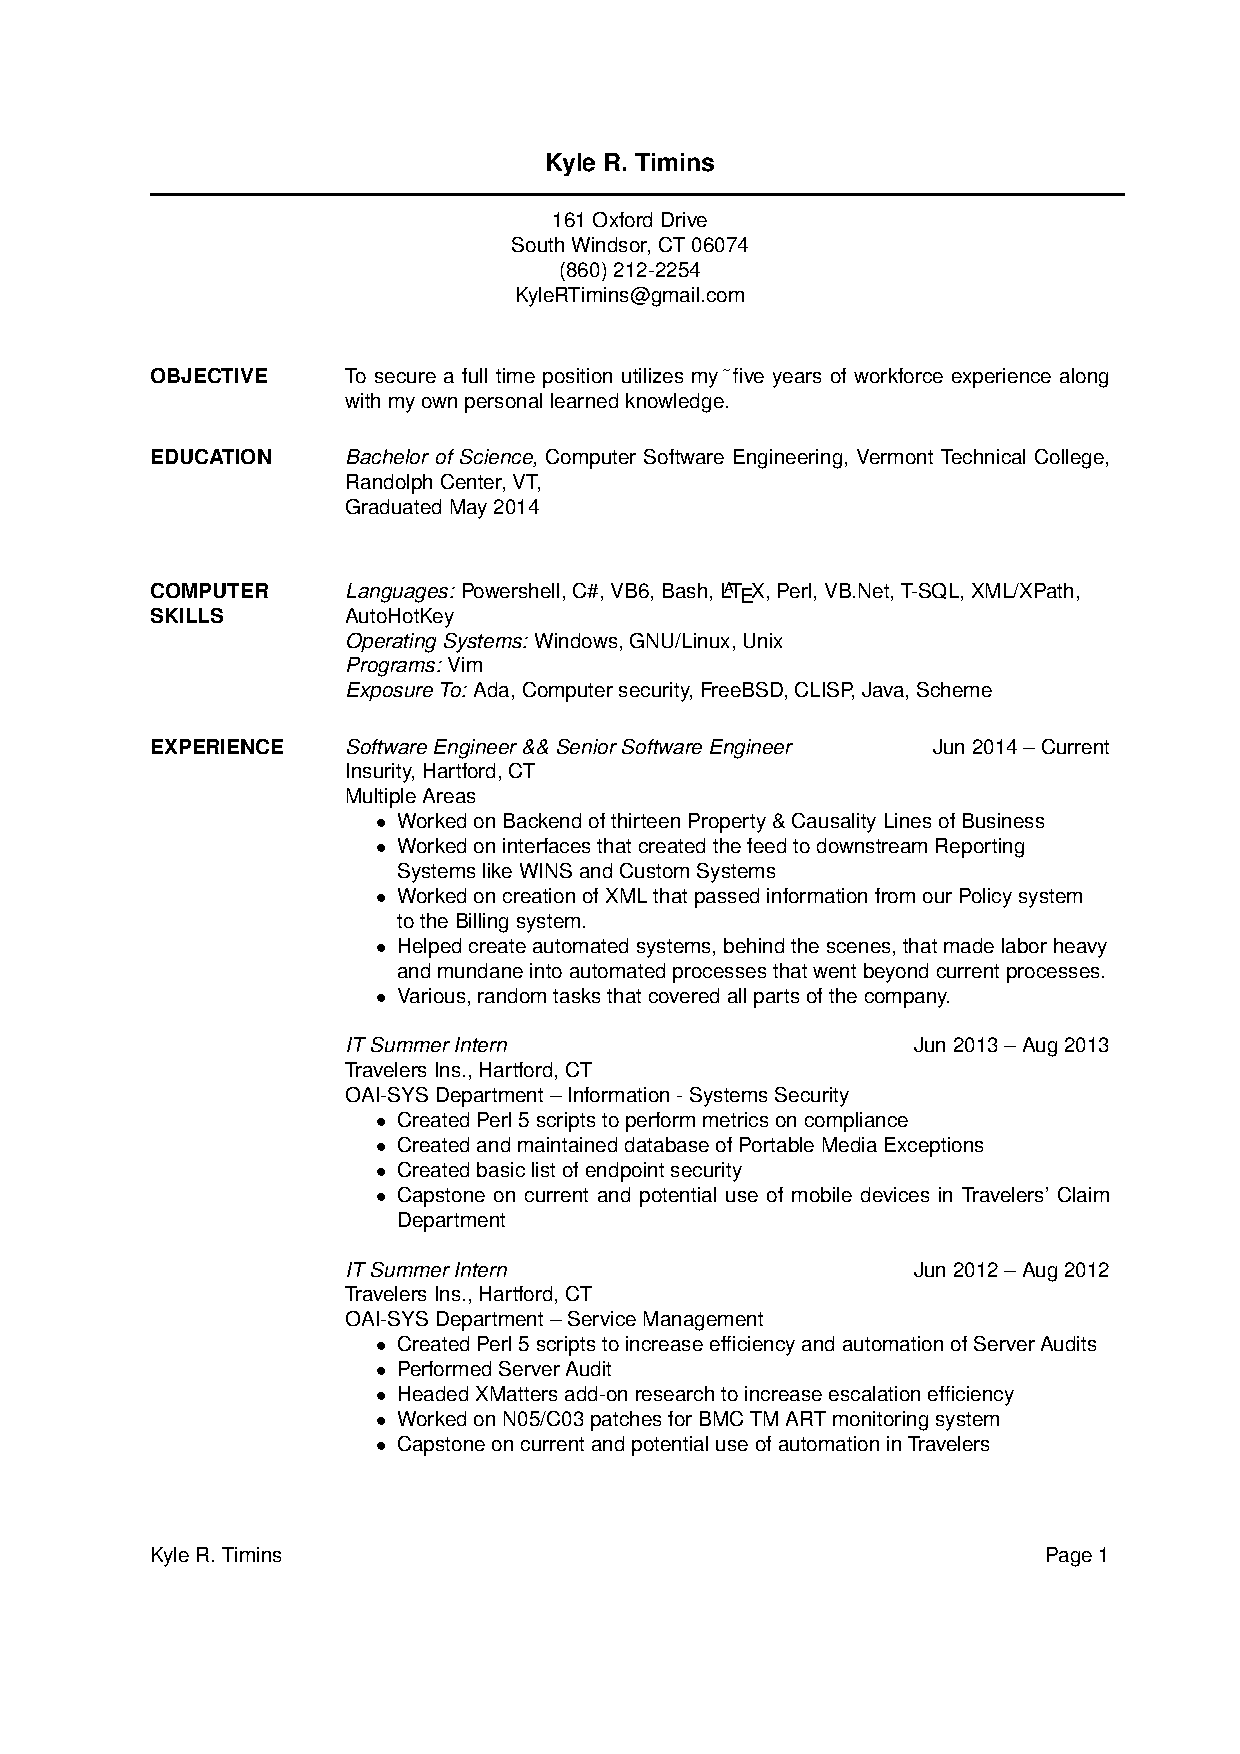
\includepdf[pages={1,2}]{Resume.pdf}
\vfill
\end{document}
